\iffalse
Title: Monoids. What, how and why?
Titulo: Monoides. Que, Como e Por Que?

Abstract:
We will learn about Monoids, a concept invented (discovered?) by mathematicians
that we can leverage to great value in our code and designs.

The talk is structured in two sessions, in this first one (5/29) we'll learn what
Monoids are, go through many examples, and write code that creates and uses Monoids. In
the second session (June maybe?) we will see how we can use Monoids to guide software design.

Despite the weird name, Monoids are easy to understand, and once you do, you'll
start finding them everywhere. More importantly, after a little practice
you'll gain intuition and you'll be able to integrate Monoids in your code and
designs, obtaining more abstract and reusable results.

Requirements:
This is an intermediate level talk. No knowledge of math or functional
programming is required. I'll assume you can understand simple Scala code.
In particular, if you don't know what implicit parameters are, spend 10 minutes
learning about them. You don't need to understand the details of implicit search
mechanisms or anything like that.


Resumo:
Vamos aprender sobre Monoids, um conceito inventado (ou descoberto?) pelos
matematicos, que nos podemos aproveitar com grandes resultados no nosso codigo e desenhos.

A palestra esta estruturada em duas sessoes, na primeira (29/05) vamos aprender o
que sao os Monoids, ver muitos exemplos e escrever codigo que cria e usa
Monoids. Na segunda sessao (data a confirmar) vamos ver como podemos usar os
Monoids para guiar o desenho de software.

Apesar de seu nome estranho, os Monoids sao faceis de entender, e uma vez que os
entenda, voce vai acha-los em todo lugar. Ainda mais importante, com um
pouco de pratica, voce vai aprimorar sua intuicao e sera capaz de integrar Monoids no seu
codigo e desenhos, consiguindo resultados mais abstratos e reusaveis.

Requerimentos:
Essa e uma palestra de nivel intermediario. Nao precisa conhecimentos de
matematica ou programacao funcional. Todos os exemplos serao em Scala, voce devera
conhecer a linguagem para entende-los. Particularmente, se voce nao sabe o que sao os parametros
implicitos, gaste 10 minutos aprendedo-os. Nao precisa saber os detalhes dos
mecanismos de busca de implicitos.

Bio:

Depois de quase uma década trabalhando em linguagens imperativas, Sebastian
abraçou a programação funcional e nunca mais olhou para atrás. Nos últimos oito anos
ele tem trabalhado nas áreas de data science, infraestrutura de Big Data e
enterprise software, em linguagens como Scala, Haskell e Clojure. Cuidado! O Sebastian vai tentar trazer você para o mundo da programação funcional.

\fi

\documentclass{beamer}

\mode<presentation>
{
  \usetheme{Madrid}      % or try Darmstadt, Madrid, Warsaw, ...
  \usecolortheme{default} % or try albatross, beaver, crane, ...
  \usefonttheme{default}  % or try serif, structurebold, ...
  \useoutertheme{default}
  \setbeamertemplate{navigation symbols}{}
  \setbeamertemplate{caption}[numbered]
  \logo{\includegraphics[height=0.8cm]{assoc2.png}}
}


\usepackage[english]{babel}
\usepackage[utf8]{inputenc}
\usepackage{listings}
\usepackage{color}
\usepackage{ulem} % for \sout
\usepackage{tikz}
\usepackage{amsmath}

\title[Monoids]{MONOIDS}
\subtitle{\textit{What}, \textit{How} and \textit{Why}}
\author{Sebastian Galkin}
\institute[@paraseba]{\texttt{@paraseba} \\ \texttt{paraseba@gmail.com}}
\date[Scaladores]{Scaladores - May 2018}

\definecolor{keyword}{rgb}{0,0.38,0}
\definecolor{comments}{rgb}{0.4,0.1,0.1}

\begin{document}
\lstset{
  language=Scala,
  basicstyle={\small\ttfamily},
  keywordstyle=\color{keyword},
  commentstyle={\color{comments}\itshape},
  columns=fullflexible,
  escapechar=~,
  showlines=false,
}


\begin{frame}
  \titlepage
\end{frame}

% Uncomment these lines for an automatically generated outline.
\begin{frame}
  \frametitle{Outline}
  \begin{columns}[c]
    \column{0.6\textwidth}
      \tableofcontents
    \column{0.4\textwidth}
      \rotatebox{45}{\Large \textcolor{blue}{\texttt{There will be quizzes}}}
  \end{columns}
\end{frame}


\begin{frame}
  \frametitle{About me}

  {\LARGE Sebastian Galkin}

  \begin{itemize}
  \item \alert{Functional Programming} for a while.
  \item Mostly \structure{big} data and enterprise.
  \item People are still scared of FP.
  \item You or your team want to learn FP?
  \color{blue}\texttt{paraseba@gmail.com}
  \end{itemize}


\end{frame}

\section{Monoids in Math \& Programming}
\subsection{Abstraction}

\begin{frame}
  \frametitle{What is Abstraction?}
  \begin{quote}
\alert{Abstraction} is the process of extracting the underlying \alert{essence} of a concept,
removing any \alert{dependence} on real world objects, and \alert{generalizing} it so that it
has \alert{wider applications.}\\[2ex] \rightline
  {{\rm --- Wikipedia, \href{https://en.wikipedia.org/wiki/Abstraction_(mathematics)}{\underline{Abstraction (mathematics)}}}}
  \end{quote}
\end{frame}

\begin{frame}
  \frametitle{You call this abstraction?}
  \begin{quote}
    I wouldn't really think of abstraction as a mathematical concept. \\[1ex] \rightline
  {{\rm --- Fishtoaster,
      \href{https://softwareengineering.stackexchange.com/questions/16070/what-is-abstraction}{\underline{SE Stack Exchange}}}}
  \end{quote}

  \begin{quote}
    A programming abstraction is a simplified model of a problem. \\[1ex] \rightline
  {{\rm --- C. Ross,
      \href{https://softwareengineering.stackexchange.com/questions/16070/what-is-abstraction}{\underline{SE Stack Exchange}}}}
  \end{quote}

  \pause

  \begin{block}{These are not abstraction}
  \begin{itemize}
    \item Inheritance.
    \item Factoring out common code to a function.
    \item Passing to functions only what they need.
  \end{itemize}
  \end{block}

  Really, how abstract is your code?

  \begin{center}
    \LARGE
    \bfseries
  We suck at abstraction!
  \end{center}

\end{frame}

\begin{frame}
  \frametitle{Standing On the Shoulders of Giants}
  Mathematicians are the \alert{masters of abstraction.}
  \begin{itemize}
  \item Maximize generality.
  \item Analogies and analogies between analogies.
  \item Reusing whole theories.
  \item Finding ``the right'' level of abstraction.
  \end{itemize}

  \pause

  \begin{center}
    \Large
    \bfseries
  This is what they have been doing for centuries.
  \end{center}

  \begin{block}{}
  copy steal copy steal copy steal
  copy steal copy steal copy steal
  copy steal copy steal copy steal
  copy steal copy steal copy steal
  copy steal copy steal copy steal
  copy steal copy steal copy steal
  copy steal copy steal copy steal
  \end{block}

\end{frame}


\subsection{What is a Monoid}

\begin{frame}
  \frametitle{What Is a Monoid?}
  \begin{block}{Monoid}
    A \alert{set} together with an \alert{associative} \alert{operation}
    and an \alert{identity} element.
  \end{block}

  \pause

  \begin{block}{Components - A Triplet \((A, \bullet, u)\)}
  \begin{itemize}
    \item A [carrier] set (\(A\))
    \item A binary operation (\(\bullet\))
    \item An element of the set \(u\)
  \end{itemize}
  We sometimes say ``\(A\) \emph{has} a Monoid''.
  \end{block}

  \pause
  \begin{block}{Laws (\(a,b,c \in A\))}

  \begin{description}[Commutativity:]
    \item[Closure:] \(a \bullet b\) is an element of \(A\)
    \item[Associativity:] \((a \bullet b) \bullet c = a \bullet (b \bullet c)\)
    \item[Identity:] \(u \bullet a = a \bullet u \ = a\)
    \item[\sout{Commutativity:}] \(a \bullet b \neq b \bullet a\)
  \end{description}
  \end{block}
\end{frame}


\subsection{Examples in math}
\begin{frame}\frametitle{A Monoid in ``Real Life''}
  Color addition

  \begin{columns}[c]
    \column{0.7\textwidth}
      \begin{itemize}
        \item \(A\): the set of all colors
        \item \(a \bullet b\): color formed adding light of color \(b\) on top
          of light of color \(a\)
        \item \(u\): transparent color
      \end{itemize}

    \column{0.3\textwidth}

    \begin{figure}
        \centering
        \def\svgwidth{\columnwidth}
        \input{additive-color.pdf_tex}
    \end{figure}
  \end{columns}

  \begin{block}{Quiz}
  What does associativity mean?
  \end{block}

  \begin{block}{Quiz}
  Is it a commutative monoid?
  \end{block}

\end{frame}

\begin{frame}\frametitle{Examples of Monoids in Math}
  \begin{itemize}
    \item Integers under addition with zero identity.
      \[
      (a + b) + c = a + (b + c) \qquad a + 0 = 0 + a = a
      \]
    \item Reals under multiplication with 1 identity.
      \[
        (a b) c = a (b c) \qquad a \times 1 = 1 \times a = a\]
    \item Subsets of a set under union with empty identity.
      \[
        \mathcal
        (\mathcal{A} \cup \mathcal{B})\cup  \mathcal{C} = \mathcal{A}\cup  (\mathcal{B}\cup  \mathcal{C}) \qquad
        \mathcal{A} \cup \emptyset = \emptyset \cup \mathcal{A} = \mathcal{A}
      \]
    \item Spatial transformations
  \end{itemize}
  \begin{block}{Quiz}
    Positive integers under division?
  \end{block}
\end{frame}

\subsection{Examples in code}

\begin{frame}\frametitle{Basic Monoids in Programming}
  \begin{itemize}
    \item<1-> \texttt{Integer} under \texttt{(+)} with \texttt{0}.
    \item<1-> \texttt{Integer} under \texttt{(*)} with \texttt{1}.
    \item\only<1>{\texttt{Double} under \texttt{(+)} with \texttt{0}?}
         \only<2->{\alert{\sout{\texttt{Double} under \texttt{(+)} with \texttt{0}}}
           \hspace{2em}
      \( (0.1+0.2)+0.3 \neq 0.1+(0.2+0.3)\).}
    \item<3-> \texttt{Boolean} under \texttt{||} with \texttt{False}.
    \item<3-> \texttt{Boolean} under \texttt{\&\&} with \texttt{True}.
    \item<3-> \texttt{Set[A]} under \texttt{union}.
  \end{itemize}

  \begin{block}{Quiz}<3->
    \begin{itemize}
    \item Is \texttt{Set[A]/union} commutative?
    \item How about \texttt{Map[K,V]/++}?
    \end{itemize}
  \end{block}
  \end{frame}

\begin{frame}[fragile]\frametitle{Modeling Monoids in Scala}
  If the type \texttt{A} \emph{has} a monoid we need:
  \begin{itemize}
    \item a way to create an \texttt{A} from nothing,
    \item a way to combine two \texttt{A}s.
  \end{itemize}
  \pause

  \begin{block}{}
  \begin{lstlisting}
trait Monoid[A] {
  // The identity
  def zero: A

  // The associative operation
  def append(a: A, b: => A): A
}
  \end{lstlisting}
  \end{block}
  We can have more than one Monoid for the same \texttt{A}
\end{frame}

\begin{frame}[fragile]\frametitle{Optional Syntax Sugar}
  \begin{block}{}
  \begin{lstlisting}
import MonoidSyntax._  // assume this in all slides

a |+| b === implicitly[Monoid[A]].append(a,b)
  \end{lstlisting}
  \end{block}

  \begin{block}{No need to understand this code}
  \begin{lstlisting}
object Monoid {
  def apply[A:Monoid]: Monoid[A] = implicitly[Monoid[A]]
}

object MonoidSyntax {
  implicit def ToMonoidOps[A:Monoid](v: A) = new MonoidOps[A](v)
  final class MonoidOps[A:Monoid](val self: A) {
    def |+|(other: => A): A = Monoid[A].append(self, other)
  }
}
  \end{lstlisting}
  \end{block}
\end{frame}

\begin{frame}[fragile]\frametitle{Two Monoids for Ints}
  \begin{block}{}
  \begin{lstlisting}
val intAddMon = new Monoid[Int] {
  def zero: Int = 0

  def append(a: Int, b: => Int): Int =
    a + b
}

val mulMon = new Monoid[Int] {
  def zero: Int = 1

  def append(a: Int, b: => Int): Int =
    a * b
}
  \end{lstlisting}
  \end{block}
  These Monoid \alert{instances} are first class citizens
\end{frame}

\begin{frame}[fragile]\frametitle{The List Monoid}
  \begin{block}{A default (?) Monoid for Lists}
  \begin{lstlisting}
implicit def freeMon[A]: Monoid[List[A]] = new Monoid[List[A]] {

  def zero: List[A] = List()

  def append(as: List[A], bs: => List[A]): List[A] =
    as ++ bs
}
  \end{lstlisting}
  \end{block}

  \begin{block}{Quiz}
Is \texttt{freeMon} a commutative monoid?
  \end{block}
\end{frame}

\begin{frame}[fragile]\frametitle{Monoid for Tuples}
  How can we combine two tuples \texttt{(A,B)}?
  \pause

  If \texttt{A} and \texttt{B} have monoids themselves, we can \alert{combine componentwise}.

  \begin{block}{}
  \begin{lstlisting}
implicit def pairMon[A: Monoid, B: Monoid] = new Monoid[(A, B)] {
  /* ~\phantom{cit def pairMon[A: Mon}\rotatebox[origin=c]{90}{$\Rsh$}~ syntax sugar for:
     (implicit am: Monoid[A], implicit bm: Monoid[B]) */

  def zero: (A,B) =
    (Monoid[A].zero, Monoid[B].zero)

  def append(a: (A, B), b: => (A, B)): (A,B) =
    (a._1 |+| b._1, a._2 |+| b._2)
}
  \end{lstlisting}
  \end{block}

  \texttt{am} and \texttt{bm} are called \alert{evidence} or
  \alert{witnesses} of the Monoids for \texttt{A} and \texttt{B}.
\end{frame}


\begin{frame}[fragile]\frametitle{Is There a Monoid for Functions?}
  It seems hard for arbitrary functions \texttt{A => B}.
  \pause
  But how about \alert{\texttt{A => A}}?

  \begin{block}{Functions that take and return the same type}

  \begin{lstlisting}
implicit def endoMon[A] = new Monoid[A => A] {

    def zero: A => A = ~\only<3->{identity}~

    def append(f: A => A, g: => (A => A)): A => A =
      ~\only<3->{g andThen f}~
  }
  \end{lstlisting}
  \end{block}
  \begin{block}<3->{Quiz}
    \begin{itemize}
      \item Is it a commutative Monoid?
      \item Can we do \texttt{(f andThen g)} instead?
    \end{itemize}
  \end{block}
\end{frame}


\begin{frame}[fragile]
  \frametitle{A Different Monoid for Functions}
  How about \texttt{(A => B)} where \alert{\texttt{B} has a Monoid?}

  \begin{block}{Functions that return a monoidal type}
  \begin{lstlisting}
implicit def monFunMon[A, B:Monoid]: Monoid[A => B] =
  new Monoid[A => B] {

    def zero: A => B =
      _ => Monoid[B].zero

    def append(f: A => B, g: => (A => B)): A => B =
      a => f(a) |+| g(a)
}
  \end{lstlisting}
  \end{block}
  Convince yourself \texttt{append} is associative.
\end{frame}

\begin{frame}[fragile]
  \frametitle{Option Monoids}
  \begin{onlyenv}<1>
  \begin{block}{Quiz}
    Would it make sense to try to write an instance of
    \texttt{Monoid[Option]?}
  \end{block}
  \end{onlyenv}

  \begin{onlyenv}<2>
    There are several ways to combine two \texttt{Option[A]}

  \begin{block}{Taking the first \texttt{Some}}
  \begin{lstlisting}
def firstMon[A]: Monoid[Option[A]] = new Monoid[Option[A]] {

  def zero: Option[A] = None

  def append(a: Option[A], b: => Option[A]): Option[A] =
    a orElse b
}
  \end{lstlisting}
  \end{block}

  Similarly taking the last \texttt{Some}
  \begin{block}{Quiz}
    \begin{itemize}
    \item What does \texttt{firstMon} do when combining a bunch of \texttt{Options}?
    \item Is it commutative?
    \end{itemize}
  \end{block}
  \end{onlyenv}

\end{frame}


\begin{frame}[fragile]
  \frametitle{Option Wrapping a Monoidal Type}
  \begin{block}{Using the wrapped monoid}
  \begin{lstlisting}
def optionMon[A:Monoid]: Monoid[Option[A]] =
  new Monoid[Option[A]] {
    def zero: Option[A] = None   // --- weird ---

    def append(a: Option[A], b: => Option[A]): Option[A] =
      (a,b) match {
        case (a, None) => a
        case (None, b) => b
        case (Some(a), Some(b)) => Some(a |+| b)
      }
}
  \end{lstlisting}
  \end{block}

  \begin{block}{Quiz}
    \begin{itemize}
      \item Why is \texttt{zero} weird?
      \item Can we do \texttt{zero = Some(m.zero)} instead?
    \end{itemize}
  \end{block}
\end{frame}

\begin{frame} \frametitle{Recap}
  We have seen:
  \begin{itemize}
    \item Monoid definition (binary assoc operation with identity).
    \item Monoid \texttt{trait} (one type parameter,
      two methods: \texttt{zero, append})
    \item Monoids for:
      \begin{itemize}
      \item Numbers, lists, tuples (if members have monoids)
      \item \texttt{A => A} and \texttt{A => M} where \texttt{M} has a monoid
      \item \texttt{Options} (first, last and Monoid wrapper)
      \item There are many, many more.
      \end{itemize}
  \end{itemize}

  \begin{block}{}
    \centering
    But we haven't seen \alert{why} or \alert{how} to use monoids.
  \end{block}
\end{frame}

\subsection{Usage}
\begin{frame}[fragile]
  \frametitle{Simple usage examples}
  \framesubtitle{\texttt{mconcat}}

  \begin{block}{A useful little function}
  \begin{lstlisting}
def mconcat[A:Monoid](as: Traversable[A]): A =
  as.foldLeft(Monoid[A].zero)(_ |+| _)~\pause~

def sum(xs: Traversable[Int]): Int = mconcat(xs)(intAddMon)~\pause~

def ~\alert{xyz}~[A](xs: Traversable[Option[A]]): Option[A] =
  mconcat(xs)(firstMon)
  \end{lstlisting}
  \end{block}
  \begin{block}<3->{Quiz}
    What does \texttt{xyz} do?
  \end{block}
\end{frame}

\begin{frame}[fragile]
  \frametitle{Simple usage examples}
  \framesubtitle{Functional MapReduce}
  \begin{block}{Super useful: \texttt{foldMap}}
  \begin{lstlisting}
def foldMap[A, M:Monoid](f: A => M)(as: Traversable[A]): M =
  as.foldRight(Monoid[M].zero) { (x,res) => f(x) |+| res }
  \end{lstlisting}
  \end{block}

  \texttt{f} acts as the mapping phase in a MapReduce, the monoidal
  operation is the reduction step.

  \vspace{6ex}

  See \texttt{Foldable} typeclass.
\end{frame}

\begin{frame}[fragile]
  \frametitle{Composing Monoids}
  \framesubtitle{Combining predicates}
  \begin{block}{Boolean has Monoids}
  \begin{lstlisting}
  implicit val allMonoid: Monoid[Boolean] = new Monoid[Boolean] {
    def zero: Boolean = true
    def append(a: Boolean, b: => Boolean): Boolean = a && b
  }
  \end{lstlisting}
  \end{block}

  \begin{onlyenv}<1>
  \begin{block}{Quiz}
    \begin{itemize}
      \item What does \texttt{allMonoid} do?
      \item Is it really associative?
      \item Is commutative?
    \end{itemize}
  \end{block}
  \end{onlyenv}

  \begin{onlyenv}<2->
    Then predicates have Monoids remember?

    \texttt{def monFunMon[A, B:Monoid]: Monoid[A => B]}
  \end{onlyenv}

  \begin{onlyenv}<3->
  \begin{block}{}
  \begin{lstlisting}
  val numbers = 1.to(100).filter(
    // type annotations needed
    (_ % 2 == 0) |+| (_ >= 10) |+| (_ < 20)
  )
  \end{lstlisting}
  \end{block}
  \end{onlyenv}
\end{frame}

\begin{frame}[fragile]
  \frametitle{Composing Monoids}
  \framesubtitle{A Monoid to compute min/max. A technique based on types.}
  \begin{block}{}
  \begin{lstlisting}
sealed abstract class Min[A]
final case class EmptyMin[A]() extends Min[A]
final case class MinValue[A](value: A) extends Min[A]

object Min {
  def apply[A](a: A): Min[A] = MinValue(a)

  // ~\phantom{   }~ Why do we need this?   ~\rotatebox[origin=c]{-90}{$\Rsh$}~
  implicit def minMonoid[A:Ordering] = new Monoid[Min[A]] {~\pause~
    def zero = EmptyMin()

    def append(a: Min[A], b: => Min[A]): Min[A] = (a, b) match {
      case (EmptyMin(), x) => x
      case (x, EmptyMin()) => x
      case (MinValue(x), MinValue(y)) => Min(List(x,y).min)
    }
  \end{lstlisting}
  \end{block}
\end{frame}

\begin{frame}[fragile]
  \frametitle{Composing Monoids}
  \framesubtitle{A Monoid to compute min/max}

  \begin{onlyenv}<1>
  \begin{block}{Calculate \texttt{min}}
  \begin{lstlisting}
def min[A: Ordering](as: Traversable[A]): Option[A] = {
  def mapper(a: A) = Min(a)

  foldMap(mapper)(as) match {  // map and reduce
    case MinValue(x) => Some(x)
    case _ => None
  }
}
  \end{lstlisting}
  \end{block}
  \end{onlyenv}

  \begin{itemize}
    \item \texttt{Min} type is hidden from \texttt{min} user.
    \item We can do the same for \texttt{Max}
  \end{itemize}
\end{frame}


\begin{frame}[fragile]
  \frametitle{Composing Monoids}
  \framesubtitle{A Monoid to compute min/max}
  \begin{block}{Calculate \texttt{min} \& \texttt{max} in a \alert{single pass}}
  \begin{lstlisting}
def minmax[A: Ordering](as: Traversable[A]): Option[(A,A)] = {
  def mapper(a: A) = (Min(a), Max(a))

  foldMap(mapper)(as) match {  // map and reduce
    case (MinValue(x), MaxValue(y)) => Some((x,y))
    case _ => None
  }
}
  \end{lstlisting}
  \end{block}

  \begin{itemize}
    \item Note how easily the Monoids \alert{compose}.
    \item Can extend to more \alert{aggregates} \texttt{(min,max,sum,size)}.
  \end{itemize}
\end{frame}

\iffalse
\begin{frame}[fragile]
  \frametitle{Composing Monoids}
  \begin{block}{Define a comparison}
  \begin{lstlisting}
sealed trait Ord[A] {
  def compare(a: A,  b:A): ~\alert{\texttt{\only<1>{??? // Scala uses Int}\only<2>{Ordering}}}~
}~\pause~

sealed trait Ordering

object Ordering {
  case object LT extends Ordering
  case object GT extends Ordering
  case object EQ extends Ordering
}
  \end{lstlisting}
  \end{block}
\end{frame}

\begin{frame}[fragile]
  \frametitle{Composing Monoids}
  \begin{block}{An \texttt{Ordering} monoid}
  \begin{lstlisting}
val ordMon = new Monoid[Ordering] {
  def zero: Ordering = Ordering.EQ

  def append(a: Ordering, b: => Ordering): Ordering =
    a match {
      case Ordering.EQ => b
      case o => o
  }
}
  \end{lstlisting}
  \end{block}
\end{frame}

\begin{frame}[fragile]
  \frametitle{Composing Monoids}
  \begin{block}{}
  \begin{lstlisting}
def sortBy(as: Array[A])(by: (A,A) => Ordering): Array[A] = ... ~\pause~
def comparing[A: Ord, B](f: B => A)(b1: B, b2: B): Ordering ~\pause~

case class Person(addr: Address, name: String, dob: Date)
case class Address(zip: Int, street: String) ~\pause~

val sorted = sortBy(people)(mconcat(List(
  comparing(_.address.zip),
  comparing(_.name),
  comparing(_.dob)))

  \end{lstlisting}
  \end{block}
\end{frame}
\fi

\begin{frame}
  \frametitle{Composing Monoids}
  Monoids compose extremely well.
  \begin{itemize}
    \item \texttt{A: Monoid}
    \item \texttt{B: Monoid}
      \pause
    \item \texttt{Option[B]: Monoid}
      \pause
    \item \texttt{(A, Option[B]): Monoid}
    \item \texttt{List[(A, Option[B])]: Monoid}
      \pause
    \item \texttt{Y => List[(A, Option[B])]: Monoid}
      \pause
    \item \texttt{X => Y => List[(A, Option[B])]: Monoid}
    \item \texttt{Map[String, X => Y => List[(A, Option[B])]]: Monoid}
  \end{itemize}
  \begin{block}{}
    \centering
    \Large \textbf{Sign of a good abstraction}
  \end{block}
\end{frame}

\begin{frame}
  \frametitle{Larger Use Cases}
  \framesubtitle{Parallelization}
  \begin{block}{The Problem}
    \begin{itemize}
      \item \texttt{append} for \texttt{Monoid[E]} is CPU expensive?
      \item We need to \texttt{mconcat} many \texttt{E}'s.: \(a_1 \bullet a_2 \bullet a_3 \dotsb \bullet a_n\)
    \end{itemize}
  \end{block}

\pause
\begin{center}
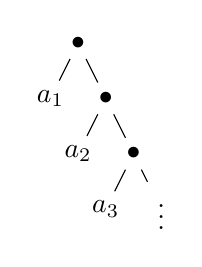
\begin{tikzpicture}[sibling distance=2em, level distance=2em]
  \node {\(\bullet\)}
    child { node {\(a_1\)} }
    child { node {\(\bullet\)}
      child { node {\(a_2\)}}
      child { node {\(\bullet\)}
        child { node {\(a_3\)}}
        child { node {\(\vdots\)}
    }}};
\end{tikzpicture}
\qquad
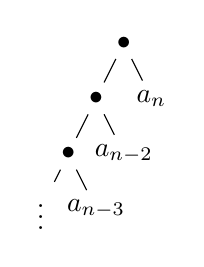
\begin{tikzpicture}[sibling distance=2em, level distance=2em]
  \node {\(\bullet\)}
    child { node {\(\bullet\)}
      child { node {\(\bullet\)}
        child {node {\(\vdots\)}}
        child {node {\(a_{n-3}\)}}}
      child { node {\(a_{n-2}\)}}
        }
    child { node {\(a_n\)} };
\end{tikzpicture}
\qquad
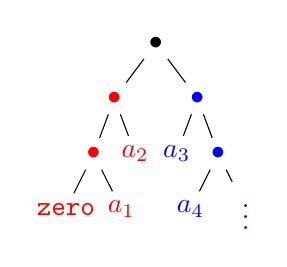
\begin{tikzpicture}[level distance=2em, level 3/.style={sibling distance=2em}, level 2/.style={sibling distance=1.5em}, level 1/.style={sibling distance=3em}]
  \node {\(\bullet\)}
  child { node[color=red] {\(\bullet\)}
    child { node[color=red] {\(\bullet\)}
      child {node[color=red] {\texttt{zero}}}
      child {node[color=red] {\(a_1\)}}}
    child { node[color=red] {\(a_2\)}}
  }
  child { node[color=blue] {\(\bullet\)}
    child { node[color=blue] {\(a_3\)} }
    child { node[color=blue] {\(\bullet\)}
      child { node[color=blue] {\(a_4\)}}
      child { node[color=blue] {\(\vdots\)}
      }}};
\end{tikzpicture}
\end{center}

\begin{block}{Quiz}
  Can we swap the two red branches in the last tree?
\end{block}
\end{frame}

\begin{frame}[fragile]
  \frametitle{Larger Use Cases}
  \framesubtitle{Parallelization}

  \begin{block}{}
  \begin{lstlisting}
object Parallel {

  def mconcat[A:Monoid](as: Traversable[A]): A =
    ~\alt<1>{as.foldLeft(Monoid[A].zero)(\_ |+| \_)}{}\alt<2>{as.\alert{fold}(Monoid[A].zero)(\_ |+| \_)}{}\alt<3->{as.\textcolor{blue}{par}.\alert{fold}(Monoid[A].zero)(\_ |+| \_)}{}~
}
  \end{lstlisting}
  \end{block}

  \invisible<1>{
    \texttt{fold[A1 >: A](z: A1)(op: (A1, A1) => A1): A1}
    \vspace{2ex}

    \texttt{z}: a \alert{neutral} element for the fold operation;
    may be added to the result an arbitrary number of times, and \alert{must not change the result.}

    \texttt{op}: a binary operator that must be \alert{associative.}
    \begin{block}{}
      \centering
      \large \textbf{But, but... That's just a Monoid!}
    \end{block}
  }
\end{frame}

\begin{frame}[fragile]
  \frametitle{Larger Use Cases}
  \framesubtitle{Parallelization}
  \begin{itemize}
    \item You could have \emph{invented} the Monoid trying to write a parallel \texttt{fold}.
    \item This is how you \emph{discover} the laws for an algebraic structure.
    \item If you have a Monoid, you can \alert{fold it in parallel.}
    \item But pay attention to the \alert{monoid laws!!!}
    \item Huge performance win (in certain situations).
    \item Base of several parallel and distributed frameworks.
  \end{itemize}

\end{frame}


\begin{frame}
  \frametitle{Larger Use Cases}
  \framesubtitle{Incremental updates}
  \begin{block}{The Problem}
    \begin{itemize}
      \item System measures a magnitude (e.g. latency)
      \item Compute and store daily means, variances, etc.
      \item Events arrive at high rate (millions per hour)
    \end{itemize}
  \end{block}


\end{frame}

\begin{frame}
  \frametitle{Larger Use Cases}
  \framesubtitle{Incremental updates}
  \begin{columns}[c]
    \column{0.6\textwidth}
      \begin{block}{Naive approach}
        \begin{itemize}
        \item On each measurement load all history,
        \item recompute mean/variance/etc.,
        \item store.
        \end{itemize}
      \end{block}

    \column{0.3\textwidth}
  Too much \alert{memory}, to much compute \alert{time}, not able to \alert{catch up}
  to the stream.
  \end{columns}

  \pause

  \begin{columns}[c]
    \column{0.6\textwidth}
      \begin{block}{Unsound approach}
        \begin{itemize}
        \item Store previous mean/variance,
        \item on measurement average previous and current,
        \item store.
        \end{itemize}
      \end{block}

    \column{0.3\textwidth}
    Fast, low memory, but \alert{incorrect}.
    \begin{align*}
      \mu[1,0,0] & = 1/3 \\
      \mu[\mu[1,0], 0] &= 1/4
    \end{align*}

  \end{columns}
\end{frame}

\begin{frame}
  \frametitle{Larger Use Cases}
  \framesubtitle{Incremental updates}
  \begin{block}{A better approach}
  \begin{itemize}
    \item Find a \alert{Monoid for mean/variance/etc} of \(n\) samples.
    \item Serialize the Monoid to storage.
    \item Accumulate several (or 1) new measurements.
    \item \alert{Combine} the old and new results using the monoid.
    \item Store.
  \end{itemize}
  \end{block}

  \pause

  \begin{block}{How is it better?}
  \begin{itemize}
    \item \alert{Exact} if we can find the right Monoid.
    \item \alert{\(O(1)\) updates} (independent of sample size).
    \item Trade off performance for freshness.
  \end{itemize}
  \end{block}

\end{frame}

\begin{frame}
  \frametitle{Larger Use Cases}
  \framesubtitle{Incremental updates}
  What to store?
  \begin{block}{Weighted average of the means}
    \[
    \begin{split}
      n\cdot \mu = \sum_{i=0}^{n-1} x_i \qquad  m\cdot \nu = \sum_{i=0}^{m-1} x_{i+n} \\
      \frac{1}{n+m} \sum_{i=0}^{n+m-1} x_i = \frac{n\mu + m\nu} {n+m}
    \end{split}
    \]
  \end{block}

  We need previous \alert{mean} and \alert{sample size.}

  Generalizing, to compute the nth-moment, we need to store n+1 values.
\end{frame}

\begin{frame}[fragile]
  \frametitle{Larger Use Cases}
  \framesubtitle{Incremental updates}
  \begin{block}{A data type for mean and variance}
  \begin{lstlisting}
sealed abstract class MeanVar

final case object EmptyMeanVar extends MeanVar

final case class MeanVarV(
  m1: Double,
  m2: Double,
  n: Long) extends MeanVar
  \end{lstlisting}
  \end{block}
\end{frame}

\begin{frame}[fragile]
  \frametitle{Larger Use Cases}
  \framesubtitle{Incremental updates}
  \begin{block}{Utility functions: creating \texttt{MeanVars}}
  \begin{lstlisting}
object MeanVar {

  def singleton(x: Double): MeanVar = MeanVarV(x, 0, 1)

  def sample(xs: Traversable[Double]): MeanVar = ~\pause~
    foldMap(singleton(_))(xs)
}
  \end{lstlisting}
  \end{block}
\end{frame}

\begin{frame}[fragile]
  \frametitle{Larger Use Cases}
  \framesubtitle{Incremental updates}
  \begin{block}{Utility functions: extracting from \texttt{MeanVars}}
  \begin{lstlisting}
object MeanVar {
  def sampleSize: MeanVar => Long = {
    case MeanVarV(_, _, n) => n
    case _ => 0
  }
  def mean: MeanVar => Option[Double] = {
    case MeanVarV(m1, _, _) => Some(m1)
    case _ => None
  }
  def variance: MeanVar => Option[Double] = {
    case MeanVarV(_, _, 1) => Some(0)
    case MeanVarV(_, m2, n) => Some(m2/(n - 1.0))
    case _ => None
  }
}
  \end{lstlisting}
  \end{block}
\end{frame}

\begin{frame}[fragile]
  \frametitle{Larger Use Cases}
  \framesubtitle{Incremental updates}
  \begin{block}{The Monoid}
  \begin{lstlisting}
val meanVarMonoid: Monoid[MeanVar] = new Monoid[MeanVar] {
  def zero: MeanVar = EmptyMeanVar

  def append(a: MeanVar, b: => MeanVar): MeanVar = (a, b) match {
    case (EmptyMeanVar, a) => a
    case (a, EmptyMeanVar) => a ~\pause~
    case (MeanVarV(m1a, m2a, na), MeanVarV(m1b, m2b, nb)) => {
      val nt = na + nb
      val delta = m1b - m1a
      MeanVarV(~\alert{(na * m1a + nb * m1b ) / nt}~,
                m2a + m2b + delta * delta * na * nb / nt,
                ~\alert{nt}~)
    }
  }
}
  \end{lstlisting}
  \end{block}
\end{frame}

\begin{frame}[fragile]
  \frametitle{Larger Use Cases}
  \framesubtitle{Incremental updates}
  \begin{block}{Updating the statistics (pseudocode)}
  \begin{lstlisting}
     // Define a time resolution (accumulate for 1sec? 100ms?)
     val newData: Vector[Double] = getNewMeasurements(...)

     // Compute mean/var of the new data (incremental work)
     val newStats: MeanVar = MeanVar.sample(newData)

     // This is an O(1) op
     // In our example this loads 3 numbers,
     // doesn't matter how many samples we have processed before
     val oldStats: MeanVar = loadStats(...)

     // Another O(1) operation
     storeStats(oldStats |+| newStats)
  \end{lstlisting}
  \end{block}
\end{frame}


\begin{frame}
  \frametitle{Larger Use Cases}
  \framesubtitle{Incremental updates}
  \begin{itemize}
    \item You could have \emph{invented} the Monoid trying to write incremental updates.
    \item This is how you \emph{discover} the laws for an algebraic structure.
    \item Didn't we say \texttt{Double} under \texttt{(+)} is not a Monoid?
    \item Extensible to higher momenta.
    \item Extensible to approximate histograms and other fun stuff.
  \end{itemize}
  \begin{block}{Take-home quiz}
    How can we do rolling averages? We would need to \emph{delete} the older
    accumulated data.
  \end{block}
\end{frame}

\subsection{References}
\begin{frame}
  \frametitle{References}
  \begin{columns}[c]
    \column{0.7\textwidth}
      \begin{itemize}

        \item This talk: slides, all the \alert{code and many tests} \\
          \href{https://github.com/paraseba/}{\underline{https://github.com/paraseba/}} % fixme

        \item \textit{Functional Programming in Scala.}\\ Paul Chiusano \& Runar Bjarnason

        \item \textit{Why Functional Programming Matters} \\
          John Hughes.

        \item \textit{Computing skewness and kurtosis in one pass.} \\
          {\footnotesize \href{https://www.johndcook.com/blog/skewness\_kurtosis/}{\underline{https://www.johndcook.com/blog/skewness\_kurtosis/}}}

        \item Scalaz library \\
          {\href{https://github.com/scalaz/scalaz}{\underline{https://github.com/scalaz/scalaz}}}
      \end{itemize}

    \column{0.3\textwidth}

    \begin{figure}
        \centering
        \includegraphics[width=\textwidth]{functional-programming-in-scala.png}
    \end{figure}
  \end{columns}
\end{frame}

\section{Monoids in Design \color[rgb]{0.5,0.1,0.9}[next session]}


\iffalse
\begin{frame}{ToDo / Fixme}
  \begin{itemize}
    \item what happens with broken rules
    \item Monoid seems too simple but it's powerful
    \item mconcat can be parallelized, incrementally, cached
    \item dual monoid
    \item summaries
    \item substracition not a monoid
    \item where to find code/presentation
    \item mathematical building, is elegant, if you don't care about
          elegance in software what do you care about? elegance is simple (not easy)
    \item accent
    \item quizes to keep awake
    \item grammarly
    \item lazyness, is the by name argument important?
    \item integer overflow is a monoid?
    \item either monoid?
    \item monoid for config
    \item grothendieck on finding the right level of abstraction
    \item mconcat can't be defined properly without associativity
    \item mention semigroup
    \item using equality when defining monoids for functions, what it means
      equal functions
    \item monoids capture *the escence* of combining things associatively
    \item laws must be probed by hand, type system not enough
    \item topic for design session: aggregations (a la beautiful folds)
  \end{itemize}
\end{frame}
\fi

\end{document}